\newpage
\chapter{Transformation Zeitreihe zu Netzwerk}
Ziel unseres Forschungsprojektes ist es unter anderem verschiedene Algorithmen, zur Ausreißer Erkennung in Netzwerken, auf Zeitreihendaten anzuwenden. Als erstes müssen hierzu die Zeitreihen in ein Netzwerk umgewandelt werden, dieser Schritt wird in diesem Kapitel erläutert. Je nach Ausreißer-Erkennung Algorithmus, muss die Transformation leicht unterschiedlich durchgeführt werden. Aus diesem Grund wird in \autoref{chap:trsnsNeti}, \autoref{chap:trsnsMidas} und \autoref{chap:trsnsMidasR} erläutert wie die Umwandlung für die jeweiligen Algorithmen funktioniert.
\section{Netsimile}
\label{chap:trsnsNeti}
Der erste Schritt der Transformation ist, die Zeitreihe in kleinere Intervalle aufzusplitten. Anschließend kann für jedes der Intervalle ein Netzwerk berechnet werden. Die Länge des Intervalls kann als Hyperparameter an den Algorithmus übergeben werden. Je nach Zeitreihe funktionieren unterschiedliche Intervallgrößen besser oder schlechter. Insofern die Zeitreihe eine Saisonalität aufweist, kann diese bestimmt und als Intervallgröße genutzt werden.
\workTodo{Überprüfen ob Saisonalität der richtige Begriff ist.}\\
Um die einzelne Zeitintervalle in ein Netzwerk umzuwandeln, wird zunächst die Distanz zwischen den einzelnen Elementen des Zeitintervalls berechnet. Hierzu wird auf das in \citep[vgl.][S.~2-3]{10.3389/fphy.2019.00194} vorgestellte Distanzmaß zurückgegriffen. Insofern für p = 2 eingesetzt wird, handelt es sich um die euklidische Distanz. Die Abstände bilden die Kantengewichte zwischen den jeweiligen Elementen im Netzwerk. Die Elemente der Zeitreihe bilden die Knoten des Netzwerks. Die Netzwerke werden intern als Adjazenzmatrizen gespeichert.
$$D_{ij}=\left(\sum_{k} \left|v_{k}^{i}-v_{k}^{j}\right|^{p}\right)^{1/p}$$
 Im nächsten Schritt müssen die Netzwerke in CSV-Dateien gespeichert werden, sodass der  Netsimile Algorithmus die Daten einlesen kann. Dazu wird für jede Kante des Netzwerks eine  Zeile im der Datei, mit folgendem Format generiert: Ursprungsknoten, Zielknoten, Gewichtung. Für jedes Zeitintervall muss eine einzelne CSV-Datei angelegt werden. Der Netsimile Algorithmus vergleicht...

\begin{figure}[H]
	\centering
	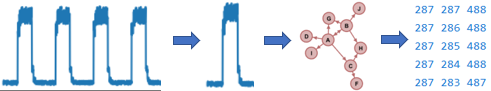
\includegraphics[width=13cm]{fig/tsToNet/tsToCsv}
	\caption{Umwandlung einer Zeitreihe in Netzwerk}
	\label{img:tsToNet}
\end{figure}
\workTodo{Das Netzwerk aus der Grafik noch abändern}



\section{MIDAS}
\label{chap:trsnsMidas}
Die Transformation der Zeitreihe in mehrere Netzwerke funktioniert für den MIDAS Algorithmus gleich wie in \autoref{chap:trsnsNeti}. Allerdings kann der Algorithmus teilweise bessere Ergebnisse erzielen, wenn für p eine Zahl größer als zwei eingesetzt wird. Dadurch werden größere Abstände zwischen Elementen stärker gewichtet.\\
Außerdem erwartet der MIDAS Algorithmus für die Netzwerkdaten ein anderes Übergabeformat. Hierbei können alle Daten der jeweiligen Zeitabschnitte in einen CSV-File geschrieben werden. Die CSV-Datei muss dabei folgendermaßen strukturiert sein: Ursprungsknoten, Zielknoten, Zeitintervall. Es ist nicht möglich die Kantengewichtung direkt an den Algorithmus zu übergeben. Um die Kantengewichtung trotzdem übergeben zu können, wird die gleiche Kante mehrmals in Abhängigkeit der Gewichtung an den Algorithmus übergeben.
Wie funkt Midas ganz kurz..


\begin{figure}[H]
	\centering
	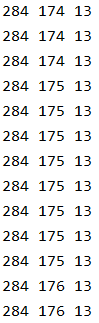
\includegraphics[width=2cm]{fig/tsToNet/midasData}
	\caption{Datensatz Midas}
	\label{img:tsToNetMiData}
\end{figure}
\workTodo{Vielleicht kleineren Auszug aus Datensatz verwenden}


\section{MIDAS-R}
\label{chap:trsnsMidasR}
\workTodo{Hab hier das mit der Hauptkomponentenzerlegung gemacht. Wenn es Ergebnisse hierfür gibt. Kann ich das hier noch erklären}
